\section{Motivation}
\begin{figure}
  \centering
   \subfloat[][An example sentence from Wiki text]{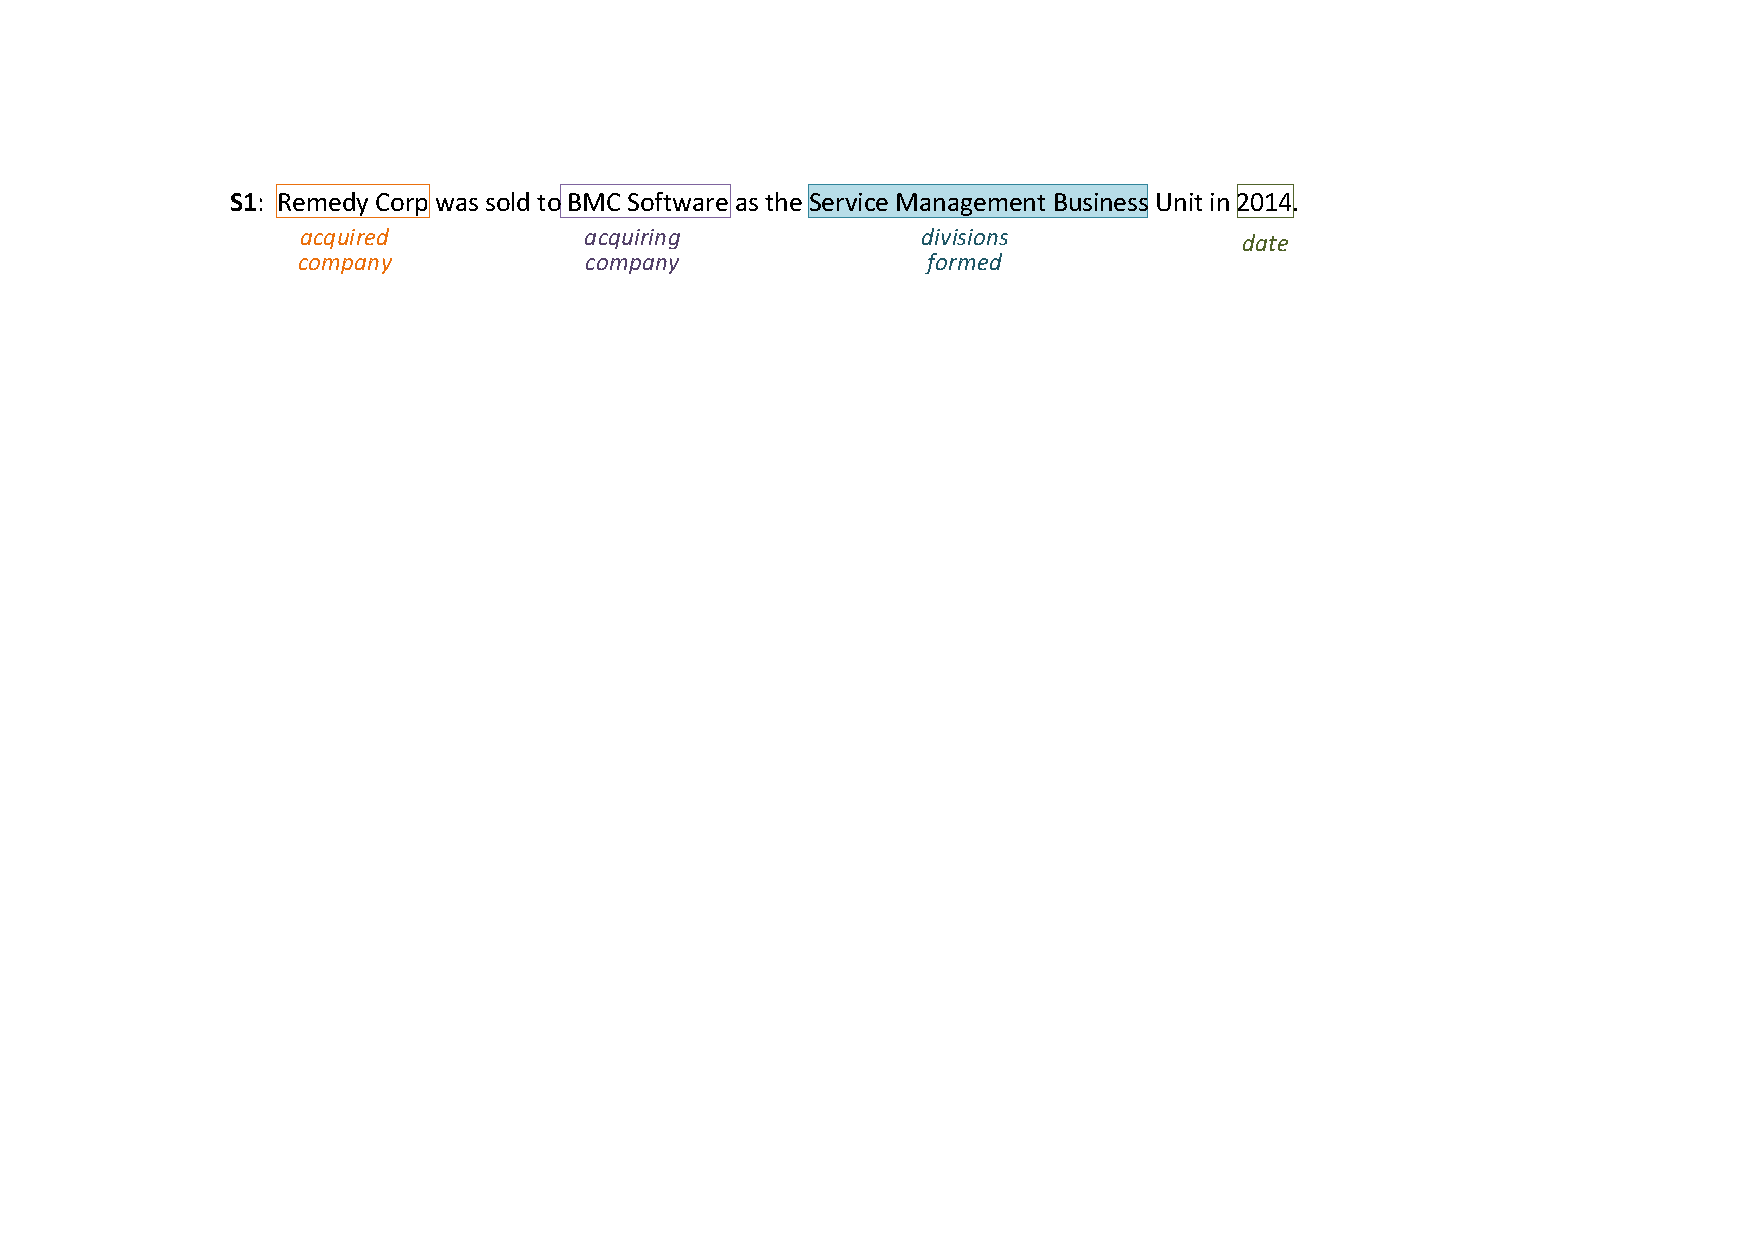
\includegraphics[width=0.5\textwidth]{figs/example.pdf}}
   \\
   \subfloat[][ Entry of \texttt{business.acquisition} in Freebase]{
        \scriptsize
        \begin{tabular}{llllp{1.6cm}}
        \toprule
        id & company\_acquired & acquiring\_company & date & divisions\_formed\\
        \midrule
        m.07bh4j7 & Remedy Corp & BMC Software & 2004 & Service Management Business Unit\\
        \bottomrule
        \end{tabular}

   }
  \caption{The event type of the sentence shown in (a) can be automatically inferred using the structured table given by Freebase in (b).}
  \label{fig:example}
\end{figure}


%The task of event extraction is to (1) detect the occurrence of events with specific types and (2) extract arguments (i.e. typed
%participants or attributes) that are associated with an event.
As a motivation example, consider a sentence from the Wiki text dataset, shown in Figure~\ref{fig:example} (a). This sentence describes a
business acquisition event. It consists of four \textbf{arguments}, \emph{company acquired} (Remedy Corp), \emph{acquiring company}
(\emph{BMC Software}), \emph{formed division} (Service Management Business Unit) and \emph{date} (2004). To learn an event extractor,
existing supervision-based approaches all require manually identifying the event type by examining the event trigger and arguments from
each individual training instance; for this examples, the trigger ``\emph{sold}" and the acquired/acquring company arguments suggest that
there is a business acquisition event.

%A predictive model is then trained, using supervised machine learning on the labelled training dataset. The model learns the
%correlation between the properties of a sentence and its corresponding event type. The learned correlations are used to predict the event
%type for new text. If we can find a way to
%automatically label training data, we can then scale up the training data generation to millions of instances instead of thousands that
%current approaches are capable of.

The problem of manually labeling is that it takes a lot of time to construct a training dataset and in many cases the resulted dataset is
too small to learn an effective event extractor. For example, it took \FIXME{man-months} to label the \FIXME{xxx} instances in the ACE
dataset. To make the learning process fast and cheap, we must take humans out of the loop of data labeling.  For this particular motivation
sentence, we discover that the structural knowledge of Freebase (\FB)~\cite{bollacker2008freebase} already provides sufficient information
to allow us to automatically label the event type. Figure~\ref{fig:example} (b) shows a Compound Value Type (\CVT) entry of \FB. A \CVT
organizes complex structured data with multiple \emph{properties} as a table\footnote{Therefore, we also use the term ``argument" to refer
to a \CVT property for the rest of the paper.}. After examining this \CVT schema, one can find that this schema implies there could be a
\emph{business.acquisition} event if the text contains properties (and arguments) like, \texttt{company\_acquired} (Remedy Corp),
\texttt{acquiring\_company} (BMC Software) and date (2004) -- all these are the identical arguments if they were extracted manually. If we
can utilize such \CVT information, we can then label the sentence shown in Figure~\ref{fig:example} (a) without needing to identify the
trigger (which is usually done by manual annotation to ensure the quality of the generated training dataset).


A natural question to ask is that ``How useful are \CVTs?". Later in this paper, we show that structured knowledge base, tables or lists
that are used to sum up certain activities can be a useful source of supervision data generation for event extraction. For example, using
just 24 \CVTs, we are able to automatically generate \FIXME{2.8 billions} \FIXME{is this true?} instances from a subset of the Wikipedia
articles (\FIXME{Section~\ref{}}).


This work develops a simple, yet effective technique to automatically generate training data by exploiting the prior \CVT knowledge from
various datasets, including \FB and Wikiedia pages. Our work shows that it is possible to scale up training data generation for event
extraction with little human involvement. In the next section, we describe g our approach of automatic traning data generation in more
details.


%%
%%Instead of asking human annotators to manually tag each individual training sentence, we use a predefine structure table to automatically
%%identify event types. In this way, experts are only required to construct a table of event types and arguments associated with each type;
%%our method can then use the table to automatically label many sentences that contains these arguments. By doing so, we essentially reduce
%%human involvement as now experts now only need to construct a table with a small number entries. \FIXME{zw: some of these need to go to
%%introduction.}  In this work, we find that structured  knowledge bases (\KB) already provide a structure table which can be used to
%%accurately infer the occurrence of certain types in real-world text.
%
%
%
%%
%%\section{The Event Extraction Task}
%%%\subsection{Event Definition}
%%% 给出相关术语的定义,subsection名字起得对吗?
%%Event extraction aims to detect the occurrence of events with specific types and extract their typed participants or attributes from text. We clarify the following terminologies within our work:
%%\begin{itemize}
%%	\item \textbf{Event mention}: a phrase or sentence within which an event is described, including its type and arguments.
%%	\item \textbf{Argument}: an entity mention, temporal expression or value that is involved in an event, with specific roles.
%%	\item \textbf{Key argument}: the argument that plays an important role in one event, and helps to distinguish with other events. % 要不要举例说明什么是key argument?这里再举例会不会和introduction里面的举例重复?
%%	% 没有地方的时候,argument role可以删掉(我看别人ACE定义的时候都讲了这个就先放上来了)
%%	%\item \textbf{Argument role}: the relationship between an event and its involved argument.
%%\end{itemize}
%
%\subsection{Indirect Supervision for Event}%{Tabular Data}
%% 缺一句连接的话?
%We first utilize Freebase~\cite{bollacker2008freebase} as a source of supervision to guide our data construction, %the structured knowledge base.
%% and there are three basics concepts: \emph{instance}, \emph{type} and \emph{property}. \emph{Instances} are entries in Freebase. \emph{Types} are different perspectives of \emph{instances}.
%where \textbf{\emph{Compound Value Type}} (CVT) is a special type to represent complex structured data % where entries are described
%with multiple \emph{properties}, usually organized in a table. Some CVT schemas indeed imply certain events, e.g., \emph{business.acquisition},
%% \emph{military.military\_service} and \emph{people.marriage},
%and closely resemble to event structures, where CVT properties can be treated as event arguments\footnote{
%Therefore, we also use the term ``argument'' to refer to CVT property in the rest of paper.}. % 直接在这里说CVT property其实就是argument,后面描述的时候不会太咯嗦
%As shown in Figure~\ref{fig:3}, the properties of CVT \emph{business.acquisition} actually can be used to label arguments of the events mentioned in S1 and S2.
%We use the Freebase copy of 2013-06,  %version of Berant et al. \shortcite{berant2013semantic},
%containing 1010 CVTs. After manually filtering out those % CVTs that
%describing Freebase structure or irrelevant to events, %(e.g., \emph{food.recipe\_ingredient})
% we obtain 24 CVTs with around 280 million instances.
%
%\begin{figure}[h]
%	\centering
%	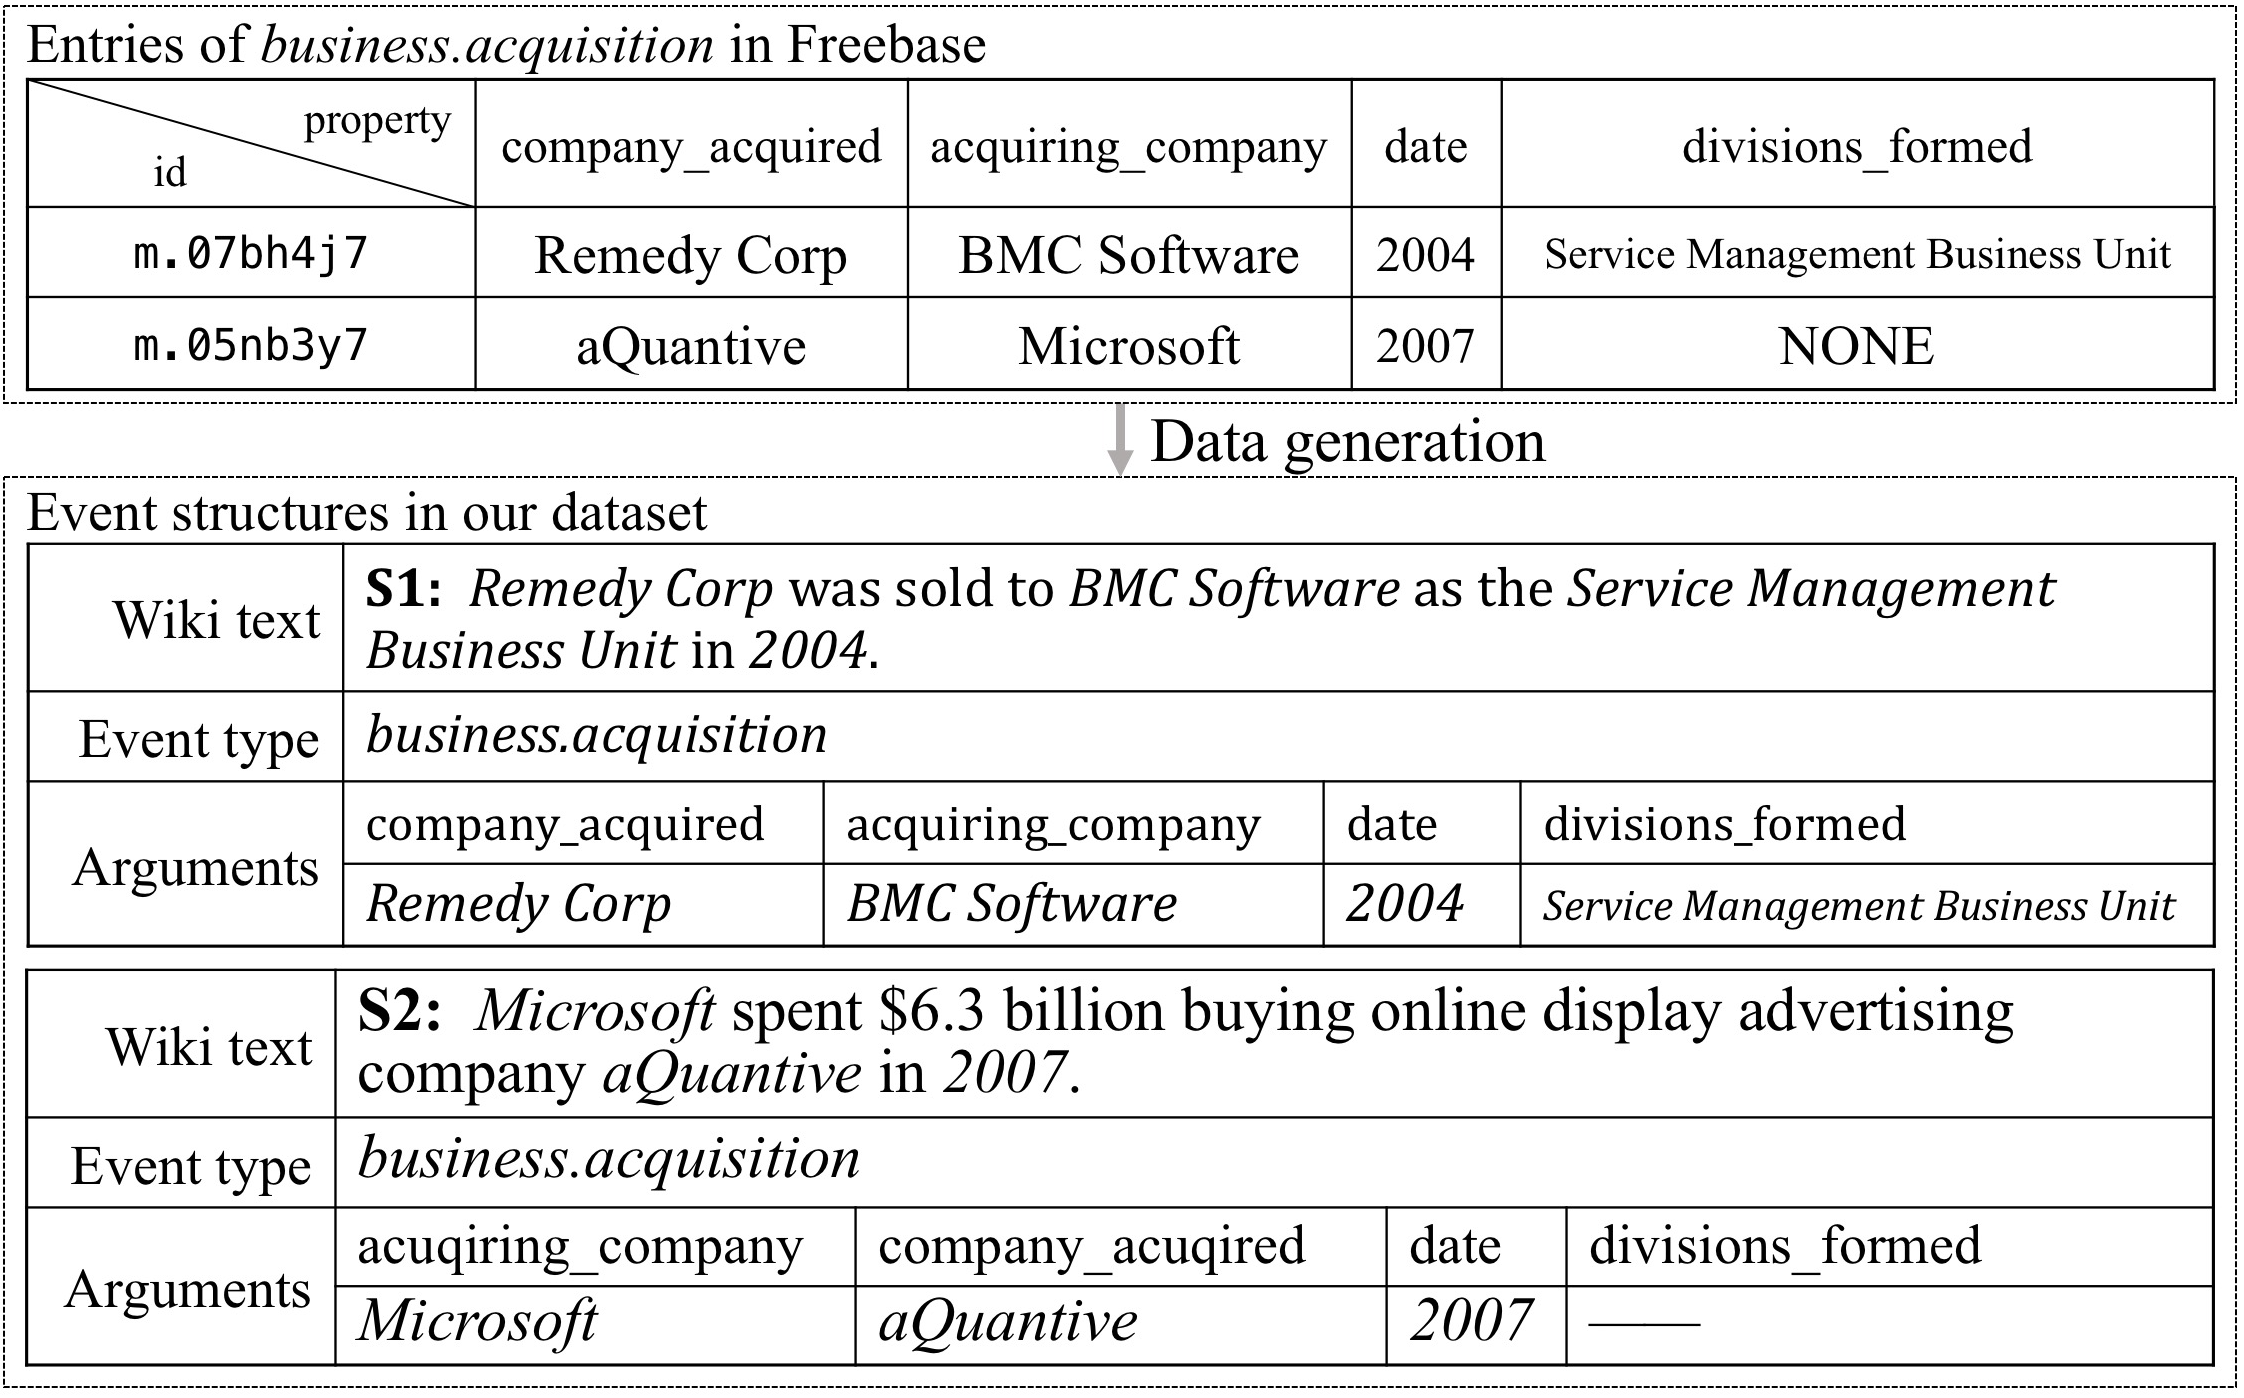
\includegraphics[width=.48\textwidth]{figure1.png}
%	\caption{Examples of a CVT table in Freebase, and labeled sentences in our dataset. \emph{Company\_acquired}, \emph{acquiring\_company} and \emph{date} are key arguments in \emph{business.acquisition}. \label{fig:3}}
%\end{figure}
%%
%Besides structured knowledge base, tables or lists that are used to sum up certain activities or occasions could be considered as a source of supervision for event extraction, as well.
%We thus investigate tables collected from Wikipedia pages, potentially referring to three types: winning of the Olympics, music and film awards, mergers and acquisitions\footnote{For example, \url{https://en.wikipedia.org/wiki/List_of_mergers_and_acquisitions_by_IBM}}.



%\subsection{Dataset Construction\label{datagen}}
%% 在哪里说其实 property 在后面就是 argument 了
%Here, we employ the event-related entries of Freebase CVT tables to illustrate how to automatically annotate event mentions in Wikipedia's articles, with the essence of distant supervision (\textbf{\texttt{DS}}): \textit{A sentence that contains \textbf{all key arguments} of an entry in an event table (e.g., CVT table) is likely to express that event}.
%%\begin{quote}
%%	\textbf{\texttt{DS}}: A sentence that contains all key arguments of an entry in an event table (e.g., CVT table) is likely to express that event in some way.
%%\end{quote}
%We will then label this sentence as a mention of this CVT event, and the words or phrases that match this entry's properties as the involved arguments, with the roles specified by their corresponding property names.
%
%We regard a sentence as \emph{positive} when it mentions the occurrence of an event, or  \emph{negative} otherwise.
%For example, S1 and S2 are positive examples with their arguments in italics and underlined (also shown in Figure~\ref{fig:3}), while S3 and S4 are negative.
%%
%\begin{quote}
%	\textbf{S1}: \underline{\emph{Remedy Corp}} was sold to \underline{\emph{BMC Software}} as the \underline{\emph{Service}} \underline{\emph{Management Business Unit}} in \underline{\emph{2004}}.
%\end{quote}
%\begin{quote}
%\textbf{S2}: \underline{\emph{Microsoft}} spent \$6.3 billion buying online display advertising company \underline{\emph{aQuantive}} in \underline{\emph{2007}}.
%\end{quote}
%\begin{quote}
%\textbf{S3}: Microsoft hopes aQuantive's Brian McAndrews can outfox Google.
%\end{quote}
%\begin{quote}
%\textbf{S4}: On April 29th, Elizabeth II and Prince Philip witnessed the marriage of Prince William.
%\end{quote}
%
%The selection strategy for key arguments of a given event type is based on two criteria: (1) \emph{Key arguments should have high importance value}; (2) \emph{Key arguments should include time-related arguments}.
%% \paragraph{H1: Positive sentences should contain all properties}
%
%% For example, S1 contains all the properties of instance $m.07bh4j7$ with a CVT type \emph{business.acquisition}, we thus consider S1 as a positive sample implying an event about \emph{business.acquisition}, and \emph{BMC Software}, \emph{Remedy Corp}, \emph{Service Management Business Unit} and \emph{2004} will be labeled as the arguments that play the role of \emph{acquiring\_company}, \emph{company\_acquired}, \emph{divisions\_formed}, and \emph{date} in this event, respectively.
%% However, in practice, we realize that \emph{H1} is too strict that excludes a great many positive sentences like S2.
%% In practice, we find that \emph{H1} is too strict to include many positive sentences like S2.
%% We thus relax \emph{H1} by replacing \textbf{all properties} with \textbf{all key properties}.
%
%The \emph{importance value} of an argument $arg$ (e.g., \emph{date}) to its event type $cvt$ (e.g., \emph{business.acquisition}) can be defined as:
%\begin{equation}
%	I_{cvt, arg} = log \frac{count(cvt, arg)}{count(cvt) \times count(arg)}
%\end{equation}
%where $count(cvt)$ is the number of instances of type $cvt$, $count(arg)$ is the number of times $arg$ appearing in all CVT types, and $count(cvt, arg)$ is the number of $cvt$ instances that contain $arg$.
%
%% We discover that for many CVTs, their key properties do not take into account time property.
%% time-related argument叫得对吗?本来的想说的是,取值为时间的argument
%Although time-related arguments are often missing in the currently imperfect KBs,
%they are indeed crucial to indicate the actual occurrence of an event, e.g., S3, containing \emph{Microsoft} as \emph{acquiring\_company} and \emph{aQuantive} as \emph{company\_acquired} but without time-related arguments, will be mistakenly considered as a positive sample for event \emph{business.acquisition}.
%% while contain all key properties of an instance, resulting in mistaking \emph{Microsoft} for \emph{acquiring\_company}, and \emph{aQuantive} for \emph{company\_acquired}.
%% By adding \emph{date} to the set of key properties, S3 will be filtered.
%
%Intuitively, two arguments involving in the same event mention are likely to be closer within the syntactic structure.
%% , which will help to eliminate negative samples.
%% We thus set the maximum distance between two key arguments as 2 empirically.
%%, i.e., for a candidate sentence, if a pair of key arguments violates this constraint, it is supposed to be negative.
%% Given the dependency parsing tree in Figure~\ref{fig:2}, S4 is negative because the distance between \emph{Prince Philip} and \emph{marriage} is 3.
%
%\begin{figure}
%\centering
%	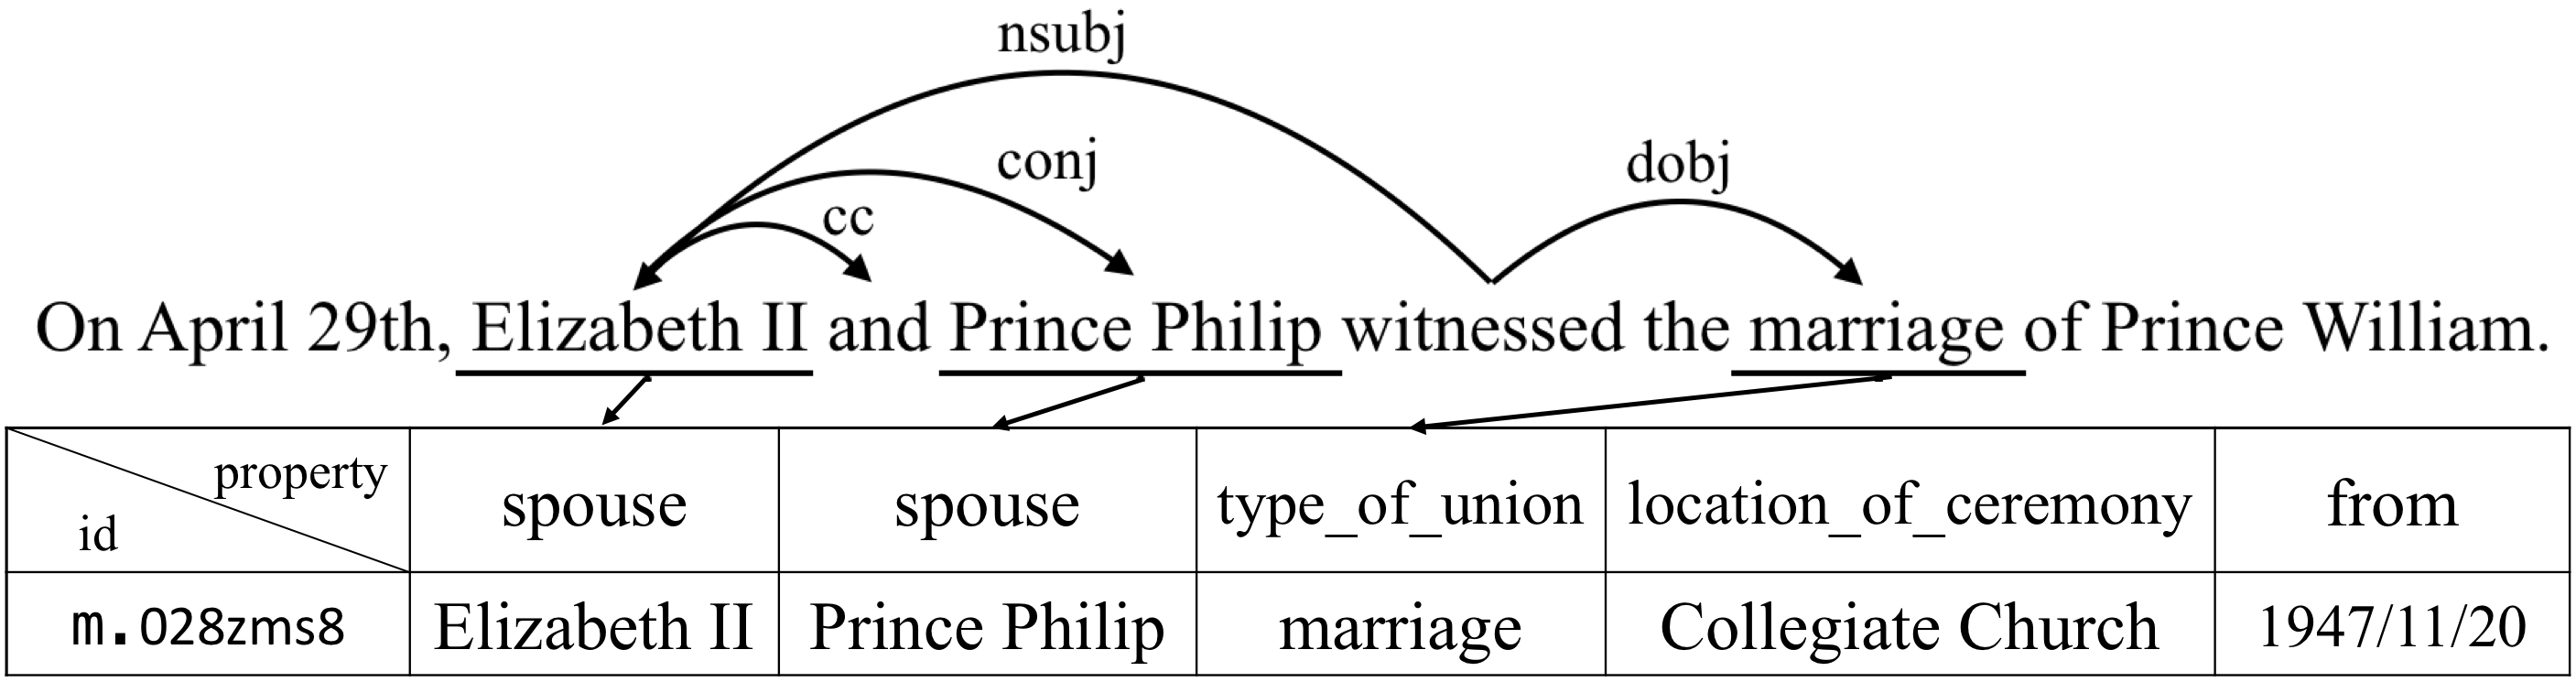
\includegraphics[width=.48\textwidth]{figure2.png}
%	\caption{The dependency tree of S4, which partially matches an entry of \emph{people.marriage}. \label{fig:2}}
%\end{figure}
%
%We conduct a series of manual evaluations on the quantity and quality of the datasets produced by different strategies (see Sec~\ref{sec:evalhypo}), and
%% following strategy produces the best dataset, thus serves as
%our final strategy is:
%for each CVT, we first sort all its arguments in descending order by their importance values, and select the top half arguments as key arguments.
%We then include the time-related argument with highest importance value as a supplementary key argument.
%Finally, we eliminate sentences in which the dependency distances between any two key arguments are greater than 2.

% 好像没地方了,先不写了
% \begin{table}
% \centering
% \small
% \begin{tabular}{|l|l|} \hline
% CVT & Key arguments \\ \hline
% award.award\_honor & award\_winner, award, \ldots, year \\ \hline
% film.performance & actor, film, character \\ \hline
% education.education & institution, student, end\_date \\ \hline
% business.employment\_tenure & company, title, person, from \\ \hline
% \end{tabular}
% \caption{Examples of key arguments of four CVTs.\label{tab:5}}
% \end{table}

%\subsection{Our Task}
%Previous event extraction systems rely on explicit trigger identification to detect the occurrence of an event,
%which is then used to decide its event type and label its arguments.
%In our automatically collected dataset, where human-labeled event triggers are unavailable, we argue that \textbf{key arguments} can play the same role as explicit event triggers.
%We thus treat the event extraction as a pipeline of the following two steps:
%\begin{itemize}
%	\item \textbf{Event detection}: to identify key arguments in a sentence. If a sentence contains \textbf{all key arguments} of a specific event type, it will be considered to imply an event mention of this specified type.
%	\item \textbf{Argument detection}: to identify other non-key arguments for each event in the sentence.
%\end{itemize}
%
%Take S1 as an example, in event detection, \emph{Remedy Corp}, \emph{BMC Software}, and \emph{2004} could be identified as \emph{company\_acquired}, \emph{acquiring\_company}, and \emph{date}, respectively, indicating that S1 may mention a \emph{business.acquisition} event.
%During argument detection, \emph{Service Management Business Unit} should be identified as \emph{divisions\_formed},
%which, together with the detected key arguments, form a full mention for a \emph{business.acquisition} event.
